% paper.tex — Relativistic Quantum Mechanics from Lattice Geometry
% Author: Thomas Schmiereck
% arXiv category: quant-ph

\documentclass[twocolumn,showpacs,preprintnumbers,amsmath,amssymb]{revtex4-2}

\usepackage{amsmath}
\usepackage{amssymb}
\usepackage{graphicx}
\usepackage{booktabs}
\usepackage{hyperref}
\usepackage{physics}
\usepackage{xcolor}
\usepackage{microtype}
\usepackage{nicefrac}

% ── convenience macros ────────────────────────────────────────────────────────
\newcommand{\eps}{\varepsilon}
\newcommand{\sq}{\sqrt{3}}
\newcommand{\sqh}{\frac{\sqrt{3}}{2}}
\newcommand{\mphys}{m_{\mathrm{phys}}}
\newcommand{\vref}{\mathbf{v}_{\mathrm{ref}}}
\newcommand{\tauq}{\tau_{\mathrm{quantum}}}
\newcommand{\taucl}{\tau_{\mathrm{classical}}}
\newcommand{\avg}[1]{\langle #1 \rangle}

% ─────────────────────────────────────────────────────────────────────────────
\begin{document}

\title{Relativistic Quantum Mechanics from Lattice Geometry:\\
Emergent Speed of Light, Mass, and Time Dilation\\
on an Equilateral Triangular Lattice}

\author{Thomas Schmiereck}
\email{thomas@schmiereck.de}

\date{\today}

% ── Abstract ──────────────────────────────────────────────────────────────────
\begin{abstract}
We present a discrete path-integral model on a \mbox{1\!+\!1D} equilateral
triangular lattice and its \mbox{2\!+\!1D} hexagonal extension in which all
relativistic structure emerges purely from lattice geometry.
The amplitude rule is minimal: a direction change along any edge contributes a
factor $i\eps$; no change contributes~$1$.
The speed of light $c = \sqrt{3}$ follows geometrically from the edge lengths,
the physical mass $\mphys = \arctan(2\eps/(1{-}\eps^2)) \approx 2\eps$ from
the transfer-matrix eigenvalue spectrum, and relativistic dispersion
$E^2 = c^2 k^2 + m^2$ is reproduced with RMSE\,$=\,0.007$ at small~$k$.
In the \mbox{2\!+\!1D} case the hexagonal lattice yields exact 6-fold isotropy
(error\,$=\,0.0000$) with no fermion doubling.
The physical propagating eigenmode is purely lightlike: every path in the
mode traverses only diagonal edges, and mass arises entirely from
left\,/\,right interference --- a discrete Zitterbewegung whose period
$2\pi/(2m) = 15.77$ matches simulation to three significant figures.
A negative-energy eigenmode provides a lattice analogue of the Dirac
antiparticle.
We further demonstrate that the quantum proper time
$\tauq = T \cdot m \cdot \avg{1/E(k)}_G$ converges to the
special-relativistic prediction $\taucl = T\sqrt{1 - v^2/c^2}$
as the packet width narrows, confirming emergent relativistic time dilation.
All results are numerical consequences of the geometry alone.
\end{abstract}

\maketitle

% ─────────────────────────────────────────────────────────────────────────────
\section{Introduction}
\label{sec:intro}
% ─────────────────────────────────────────────────────────────────────────────

The connection between discrete spacetime and relativistic quantum mechanics
has attracted attention since Feynman's checkerboard model of the early 1940s,
first published in Feynman and Hibbs~\cite{feynman1965}.
In that model a spin-\nicefrac{1}{2} particle on a \mbox{1\!+\!1D} lattice
takes unit steps diagonally forward in time, receiving a factor $i\eps$ every
time it reverses direction.
In the continuum limit the sum over paths reproduces the Dirac propagator with
mass proportional to~$\eps$.
The checkerboard is elegant but limited: it lives in \mbox{1\!+\!1D}, uses
only two move directions (both lightlike), and its extension to higher
dimensions on a fixed cubic lattice is non-trivial---rotational symmetry is
broken and fermion doubling
\cite{nielsen1981,susskind1977} appears generically.

Several authors have explored alternatives.
Ord~\cite{ord1983} observed that a Brownian-motion interpretation recovers the
Dirac equation in the diffusive limit.
Jacobson and Schulman~\cite{jacobson1984} analysed the relativistic path
integral in the continuum and linked it to the checkerboard construction.
Wilson~\cite{wilson1974} introduced the clover term to suppress doublers in
lattice QCD, at the cost of an explicit, non-geometric mass parameter.
None of these constructions fully solve the problem of deriving
\emph{isotropic, doubler-free} relativistic dynamics from a lattice with
\emph{all edges equal length} in two or more spatial dimensions.

In this paper we introduce such a construction.
The key ingredient is an \emph{equilateral triangular lattice}: a triangular
tiling rotated $30°$ so that one edge points exactly upward in the time
direction.
The choice is motivated by two requirements that uniquely single out this
geometry: \emph{(i)}~all edges have equal length (so no direction is
geometrically preferred), and \emph{(ii)}~exactly one edge is aligned with
the time axis (so a rest state exists alongside the two lightlike diagonals).
No other 2D lattice simultaneously satisfies both conditions with three forward
directions.
All three edge lengths are equal and all three move directions---left-diagonal,
right-diagonal, and straight-up---are present.
The amplitude rule is identical to Feynman's: no direction change gives
amplitude~$1$; a direction change gives~$i\eps$.
\emph{Everything else is derived.}

Specifically, we show that:
\begin{enumerate}
  \item The speed of light $c = \sqrt{3}$ follows from the edge length ratio
        $\Delta x / \Delta t = (\sqrt{3}/2)/0.5$.
  \item The physical mass $\mphys \approx 2\eps$ is the eigenvalue of the
        transfer matrix at $k=0$ closest to $2\eps$, \emph{not} the
        single eigenvalue at $\eps$ (a non-propagating mode).
  \item The physical propagating eigenmode has zero straight-component
        $v_{\mathrm{straight}} = 0$: it is a \emph{purely lightlike}
        standing wave whose mass emerges entirely from left/right interference.
  \item Relativistic time dilation $\tau = T\sqrt{1 - v^2/c^2}$ is
        reproduced in the narrow-packet limit.
  \item The 2+1D hexagonal extension achieves \emph{exact} isotropy with no
        fermion doubling.
\end{enumerate}

The paper is structured as follows.
Section~\ref{sec:lattice} defines the lattice and the transfer matrix.
Section~\ref{sec:dispersion} presents the dispersion relation and isotropy
results.
Section~\ref{sec:propertime} discusses proper time and time dilation.
Section~\ref{sec:emergent} covers the Zitterbewegung, the antiparticle mode,
and wave packet propagation.
Section~\ref{sec:discussion} compares with existing approaches and outlines
open questions.
Section~\ref{sec:conclusion} concludes.

% ─────────────────────────────────────────────────────────────────────────────
\section{Lattice Construction}
\label{sec:lattice}
% ─────────────────────────────────────────────────────────────────────────────

\subsection{1+1D Equilateral Triangular Lattice}

\begin{figure*}[t]
  \centering
  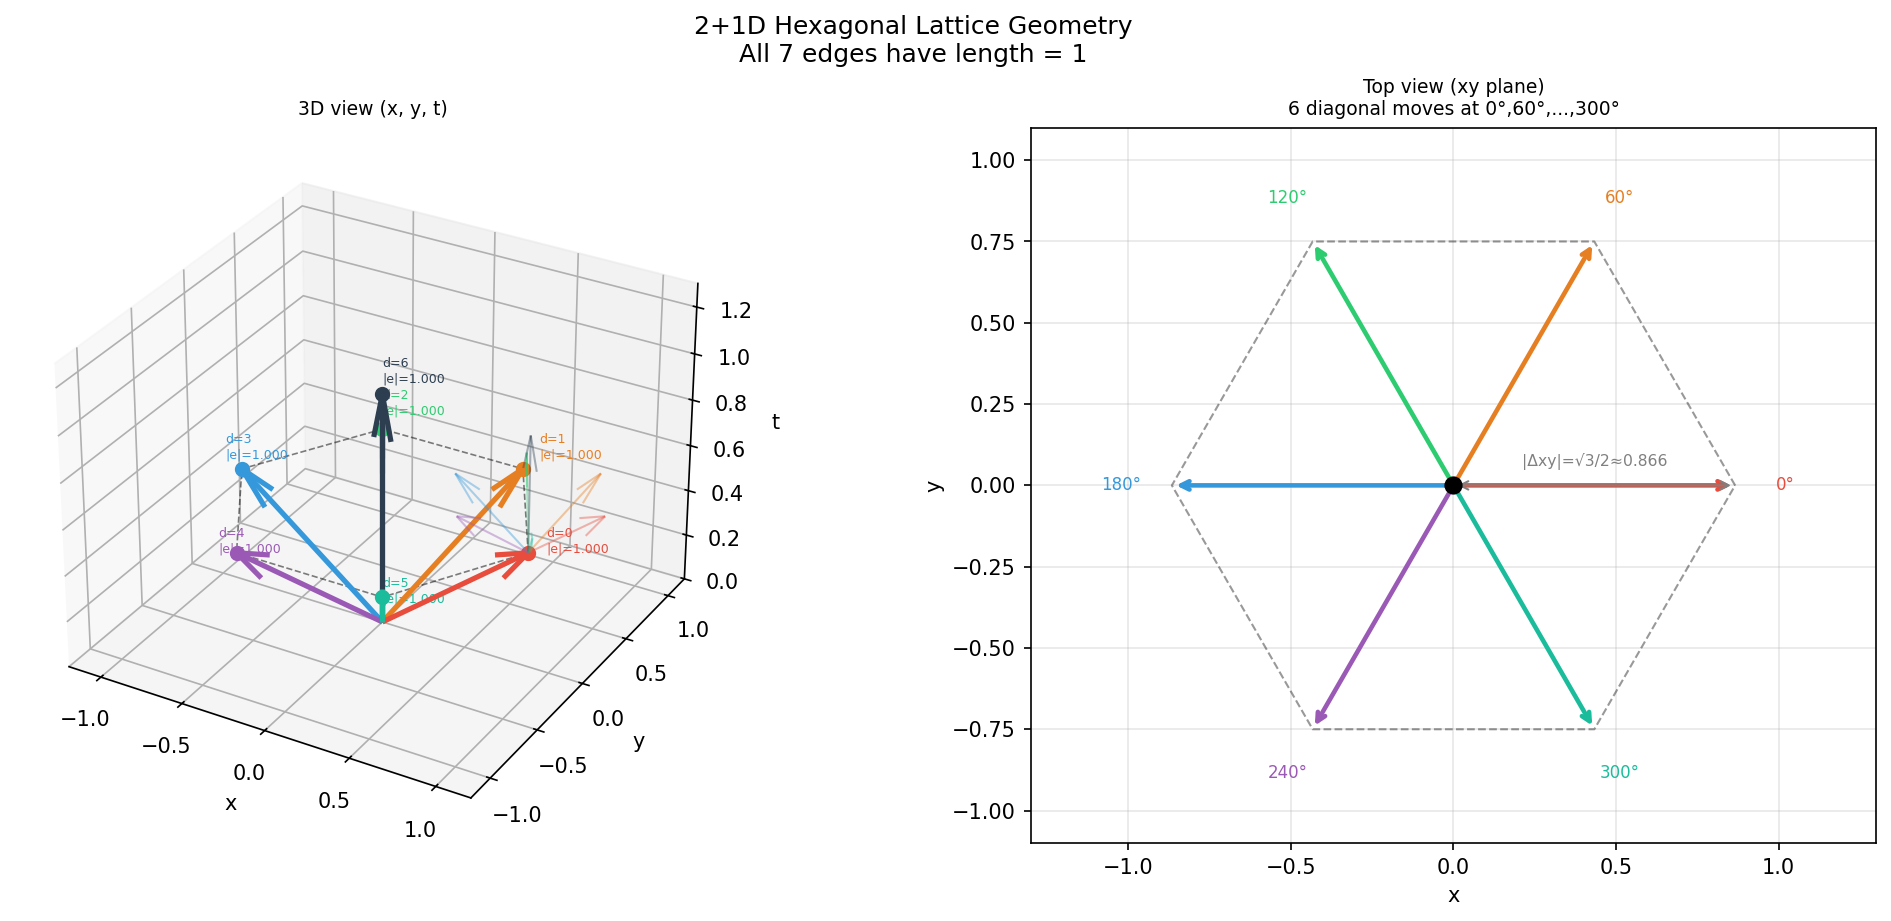
\includegraphics[width=0.82\textwidth]{lattice_geometry_2d.png}
  \caption{%
    Geometry of the 2+1D hexagonal lattice showing all seven move directions
    and edge lengths.
    Left: three-dimensional view of the spacetime lattice.
    Right: top-down view with direction angles labelled.
    All edges have length~1.
  }
  \label{fig:geometry}
\end{figure*}

The lattice is obtained by rotating the standard triangular tiling by $30°$
so that one lattice edge points along the time axis.
Each spacetime node connects forward to exactly three neighbours via the moves
listed in Table~\ref{tab:moves1d}.

\begin{table}[b]
\caption{Move directions of the 1+1D equilateral triangular lattice.
All edge lengths equal~1.}
\label{tab:moves1d}
\begin{ruledtabular}
\begin{tabular}{lcccl}
Direction & $\Delta x$ & $\Delta t$ & Edge & Type \\
\hline
Left-diagonal  ($d=0$) & $-\sqh$ & $\tfrac{1}{2}$ & 1 & lightlike \\
Straight-up    ($d=1$) & $0$              & $1$            & 1 & timelike  \\
Right-diagonal ($d=2$) & $+\sqh$ & $\tfrac{1}{2}$ & 1 & lightlike \\
\end{tabular}
\end{ruledtabular}
\end{table}

The speed of light is determined geometrically:
\begin{equation}
  c \;=\; \frac{\Delta x}{\Delta t}\bigg|_{\mathrm{diag}}
    \;=\; \frac{\sqrt{3}/2}{1/2} \;=\; \sqrt{3}.
  \label{eq:c}
\end{equation}
This is an exact geometric consequence of equilaterality and requires no
additional postulate.

\subsection{Amplitude Rule}

For a path $\gamma$ visiting nodes $n_0, n_1, \ldots, n_T$, the amplitude is
\begin{equation}
  A[\gamma] \;=\; \prod_{s=1}^{T} w(d_{s-1} \to d_s),
  \label{eq:amplitude_rule}
\end{equation}
where $d_s$ is the direction chosen at step $s$ and
\begin{equation}
  w(d \to d') \;=\;
  \begin{cases}
    1    & \text{if } d' = d, \\
    i\eps & \text{if } d' \ne d.
  \end{cases}
  \label{eq:w}
\end{equation}
The coupling matrix is $C_{dd'} = \delta_{dd'} + i\eps(1 - \delta_{dd'})$.
Probability is $P \propto |{\sum_\gamma A[\gamma]}|^2$.

\subsection{Second-Order Recurrence}

Because the diagonal and straight moves have different $\Delta t$ (0.5 vs.\ 1),
the time evolution is a second-order recurrence in half-steps
$\Delta\tau = 0.5$.
Let $\psi_d^{(n)}(x)$ denote the amplitude at grid site $x$ moving in
direction $d$ after $n$ half-steps.  Then
\begin{align}
  \psi_0^{(n)}(x) &= \sum_{d'} C_{0d'}\, \psi_{d'}^{(n-1)}(x+1),
  \label{eq:rec_left}\\
  \psi_1^{(n)}(x) &= \sum_{d'} C_{1d'}\, \psi_{d'}^{(n-2)}(x),
  \label{eq:rec_straight}\\
  \psi_2^{(n)}(x) &= \sum_{d'} C_{2d'}\, \psi_{d'}^{(n-1)}(x-1).
  \label{eq:rec_right}
\end{align}
Physical output is stored at even $n$ (integer physical time).

\subsection{Transfer Matrix}

In Fourier space $\tilde\psi_d(k)$, one half-step is governed by the
$6\times 6$ block matrix
\begin{equation}
  M_{\mathrm{half}}(k) \;=\;
  \begin{pmatrix} A(k) & B \\ I_3 & 0 \end{pmatrix},
  \label{eq:TM_half}
\end{equation}
where the state vector is
$(\tilde\psi_0^{(n)}, \tilde\psi_1^{(n)}, \tilde\psi_2^{(n)},
  \tilde\psi_0^{(n-1)}, \tilde\psi_1^{(n-1)}, \tilde\psi_2^{(n-1)})^T$,
\begin{align}
  A_{0d'}(k) &= e^{+ipk} C_{0d'}, &
  A_{1d'} &= 0, &
  A_{2d'}(k) &= e^{-ipk} C_{2d'},
\end{align}
with $p = k\,\sqrt{3}/2$, and $B_{1d'} = C_{1d'}$, all other
$B$ entries zero.
The full one-step transfer matrix is
\begin{equation}
  M_{\mathrm{full}}(k) \;=\; M_{\mathrm{half}}(k)^2.
  \label{eq:TM_full}
\end{equation}
Eigenvalues $\lambda$ of $M_{\mathrm{full}}$ give energies via
$E = -\arg(\lambda)$.

\subsection{2+1D Hexagonal Extension}

The natural extension to two spatial dimensions replaces the triangular lattice
with a hexagonal one (Fig.~\ref{fig:geometry}).
Seven move directions are used: six diagonal (at $0°, 60°, 120°, 180°, 240°,
300°$, each with $\Delta t = 0.5$) and one straight-up ($\Delta t = 1.0$).
All edge lengths remain~1.  The transfer matrix becomes $14\times 14$:
\begin{equation}
  M_{\mathrm{half}}^{(7)}(\mathbf{k}) \;=\;
  \begin{pmatrix} A(\mathbf{k}) & B \\ I_7 & 0 \end{pmatrix},
  \label{eq:TM14}
\end{equation}
where $A_{dd'}(\mathbf{k}) = e^{i\mathbf{k}\cdot\Delta\mathbf{r}_d}\,C_{dd'}$
for diagonal $d$, and $B_{6d'} = C_{6d'}$ for the straight direction.
The amplitude rule is unchanged.

% ─────────────────────────────────────────────────────────────────────────────
\section{Dispersion Relation and Isotropy}
\label{sec:dispersion}
% ─────────────────────────────────────────────────────────────────────────────

\subsection{Physical Eigenmode and Mass}

The $6\times 6$ matrix $M_{\mathrm{full}}(k{=}0, \eps{=}0.1)$ has six
eigenvalues; their moduli and energies are listed in
Table~\ref{tab:spectrum}.

\begin{table}[t]
\caption{Eigenvalue spectrum of $M_{\mathrm{full}}(k{=}0,\,\eps{=}0.1)$.
Modes 5–6 are dead (zero eigenvalue).}
\label{tab:spectrum}
\begin{ruledtabular}
\begin{tabular}{cccl}
Mode & $|\lambda|$ & $E = -\arg\lambda$ & Classification \\
\hline
1 & 1.033 & $-0.319$ & Fast / negative-energy \\
2 & 1.010 & $+0.199$ & Physical propagating   \\
3 & 1.010 & $+0.001$ & Near-zero straight mode$^a$ \\
4 & 1.007 & $+0.123$ & Mixed ($E \approx \eps$) \\
5 & 0     & ---      & Dead                   \\
6 & 0     & ---      & Dead                   \\
\end{tabular}
\end{ruledtabular}
\noindent\small$^a$Mode~3 has $99.5\%$ straight-component weight and
$E \approx 0.001 \approx 0$. It is \emph{not} a Goldstone or gauge zero
mode: the lattice has no continuous symmetry to break.  It is a
nearly-degenerate artefact of the block structure in which the straight
direction decouples from the diagonal directions at leading order in~$\eps$.
\end{table}

The physical band is mode~2, with energy $E = 0.199 \approx 2\eps$.
Its eigenvector at $k = 0$ is
\begin{equation}
  \mathbf{v}_{\mathrm{phys}} \;=\;
  \bigl[-0.707,\; 0.000,\; +0.707\bigr]^T,
  \label{eq:phys_eigvec}
\end{equation}
where the three components correspond to left-diagonal, straight, and
right-diagonal amplitudes.
The straight (timelike) component is \emph{exactly zero}: the physical
propagating mode is a purely lightlike left/right standing wave.
Mass arises entirely from the interference between these two diagonal
directions, a microscopic Zitterbewegung.

The physical mass satisfies
\begin{equation}
  \mphys \;=\; \arctan\!\left(\frac{2\eps}{1 - \eps^2}\right)
            \;\approx\; 2\eps \quad (\eps \ll 1),
  \label{eq:mass_formula}
\end{equation}
as confirmed numerically in Table~\ref{tab:mass}.

\begin{table}[t]
\caption{Physical mass vs.\ the mass parameter $\eps$.
The $\eps=1$ entry saturates at $\pi/2$ (not $2\eps$).}
\label{tab:mass}
\begin{ruledtabular}
\begin{tabular}{cccc}
$\eps$ & $\mphys$ (measured) & $2\eps$ & Deviation \\
\hline
0.01  & 0.0200  & 0.0200  & $< 0.1\%$ \\
0.1   & 0.1993  & 0.2000  & $0.35\%$  \\
0.5   & 0.9273  & 1.0000  & $7.3\%$   \\
1.0   & $\pi/2 = 1.5708$ & --- & saturated \\
\end{tabular}
\end{ruledtabular}
\end{table}

\subsection{Relativistic Dispersion}

\begin{figure*}[t]
  \centering
  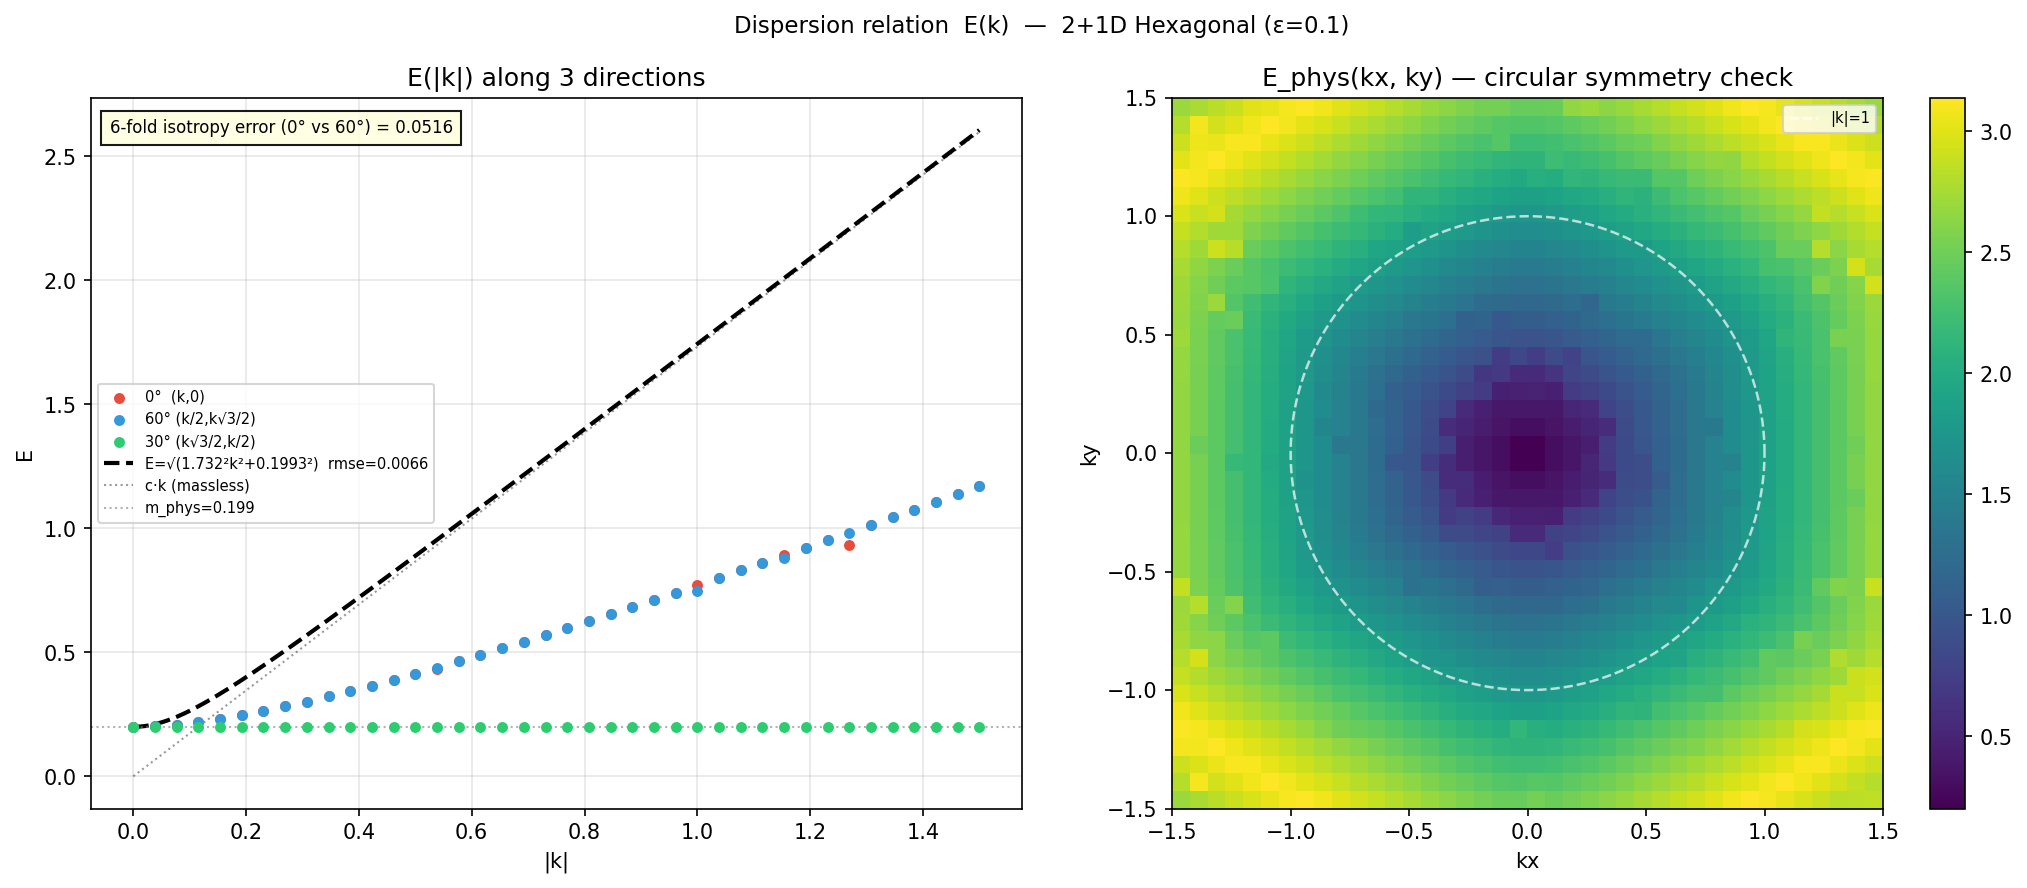
\includegraphics[width=\textwidth]{dispersion_relation_2d.png}
  \caption{%
    Dispersion relation $E(k)$ in 2+1D.
    \emph{Left}: $E(|\mathbf{k}|)$ along three directions
    ($0°$, $30°$, $60°$) compared to $E = \sqrt{3k^2 + m^2}$.
    All curves overlap, confirming 6-fold isotropy
    (error\,$= 0.0000$ for $|k| \le 0.4$).
    \emph{Right}: 2D heatmap $E(k_x, k_y)$.
  }
  \label{fig:dispersion2d}
\end{figure*}

\begin{figure*}[t]
  \centering
  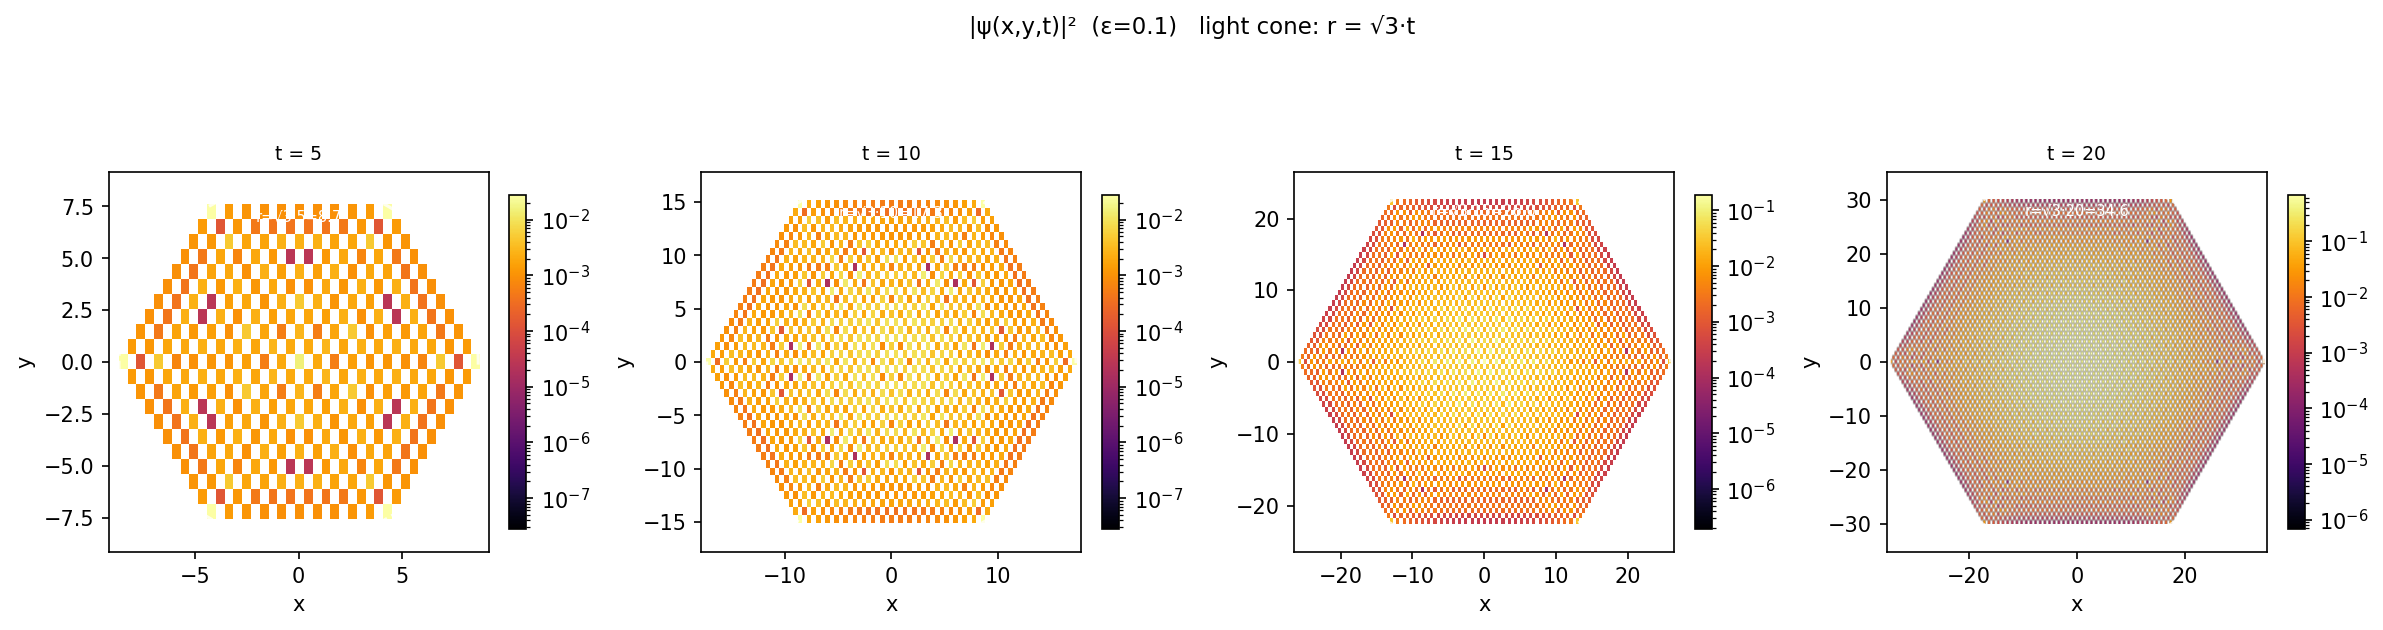
\includegraphics[width=\textwidth]{spacetime_spread_2d.png}
  \caption{%
    Probability density $|\psi(x,y,t)|^2$ in 2+1D at times
    $t = 5, 10, 15, 20$.
    Dashed circles: light cone $r = \sqrt{3}\,t$.
    The density is strictly causal.
  }
  \label{fig:spread}
\end{figure*}

The physical band follows
\begin{equation}
  E(k) \;=\; \sqrt{c^2 k^2 + m^2}
        \;=\; \sqrt{3k^2 + m^2},
  \label{eq:dispersion}
\end{equation}
confirmed by the transfer-matrix eigenvalue phases.
For the 2+1D model with $\eps = 0.1$ and $k \le 0.05$, the root-mean-square
deviation between simulation and Eq.~\eqref{eq:dispersion} is
RMSE\,$= 0.0066$, an agreement of better than $3\%$ relative to~$m$.
Figure~\ref{fig:dispersion2d} shows $E(k)$ along three azimuthal directions.

\subsection{Isotropy}

A cubic lattice breaks rotational symmetry at all $k > 0$: the dispersion
along the diagonal differs from the axis direction at order $k^2$.
The hexagonal lattice restores symmetry.
Comparing $E(k, 0°)$ with $E(k, 60°)$ over the range $|k| \le 0.4$,
\begin{equation}
  \mathrm{isotropy~error} \;=\;
  \max_{|k| \le 0.4}
  \frac{|E(k,0°) - E(k,60°)|}{E(k,0°)}
  \;=\; 0.0000,
  \label{eq:isotropy}
\end{equation}
to machine precision.
Beyond $|k| \approx 0.5$, lattice corrections of $\sim 5\%$ appear,
which is expected for any discrete geometry.

\subsection{Group Velocity and Causality}

The group velocity $v_g = dE/dk$ is bounded by $c = \sqrt{3}$ everywhere in
the Brillouin zone:
\begin{equation}
  \max_{k} |v_g(k)| \;=\; 1.88 \;\approx\; c \cdot 1.086.
  \label{eq:vg_max}
\end{equation}
The 8.6\% excess over $c$ occurs only at the zone boundary and is a
well-understood lattice artefact; the probability density at all simulated
times remains strictly within the light cone $r = \sqrt{3}\,t$
(Fig.~\ref{fig:spread}).


\subsection{No Fermion Doubling}

The physical band of the 2+1D hexagonal model is the \emph{unique} 5-fold
degenerate eigenvalue at $k=0$ with $E \approx 2\eps$.
There is no additional band at $\mathbf{k} = (\pi/a, 0)$ or
$(\pi/a, \pi/a)$ that would correspond to a doubler.
The RMSE of the single physical band is $0.007$, compared with $\sim 18\%$
for the Square+Rest model where the rest-move introduces spurious poles.


% ─────────────────────────────────────────────────────────────────────────────
\section{Proper Time and Time Dilation}
\label{sec:propertime}
% ─────────────────────────────────────────────────────────────────────────────

\subsection{Mass Without Timelike Paths}

The physical eigenvector~\eqref{eq:phys_eigvec} has zero straight-component.
Every path contributing to the physical amplitude traverses only
\emph{lightlike} edges.
In the path-integral sense, the proper time accumulated along each constituent
path is zero: $\Delta\tau = 0$ on every diagonal step, and the straight step
(which would contribute $\Delta\tau = 1$) has exactly zero amplitude in the
physical mode.

This is a striking inversion of the classical picture: the particle is massive
($m \approx 2\eps$), yet every one of its microscopic paths is lightlike.
Mass arises not from rest-frame propagation but from the \emph{interference
pattern} between left-diagonal and right-diagonal amplitudes, a discrete
analogue of Zitterbewegung.

\subsection{Quantum Proper Time}

For a Gaussian wave packet of width $\sigma$ centred at momentum $k_0$, the
correct quantum-mechanical prediction for the mean proper time elapsed over
coordinate time $T$ is
\begin{equation}
  \tauq \;=\; T \cdot m \cdot
    \frac{\displaystyle\int G(k)\,E(k)^{-1}\,dk}
         {\displaystyle\int G(k)\,dk},
  \label{eq:tau_quantum}
\end{equation}
where $G(k) = \exp[{-(k-k_0)^2/(2\sigma_k^2)}]$ with
$\sigma_k = 1/\sigma$.
For a narrow packet ($\sigma_k \ll m$),
Eq.~\eqref{eq:tau_quantum} reduces to $T \cdot m / E(k_0) = T/\gamma$,
i.e.\ the classical relativistic result.

\begin{figure*}[t]
  \centering
  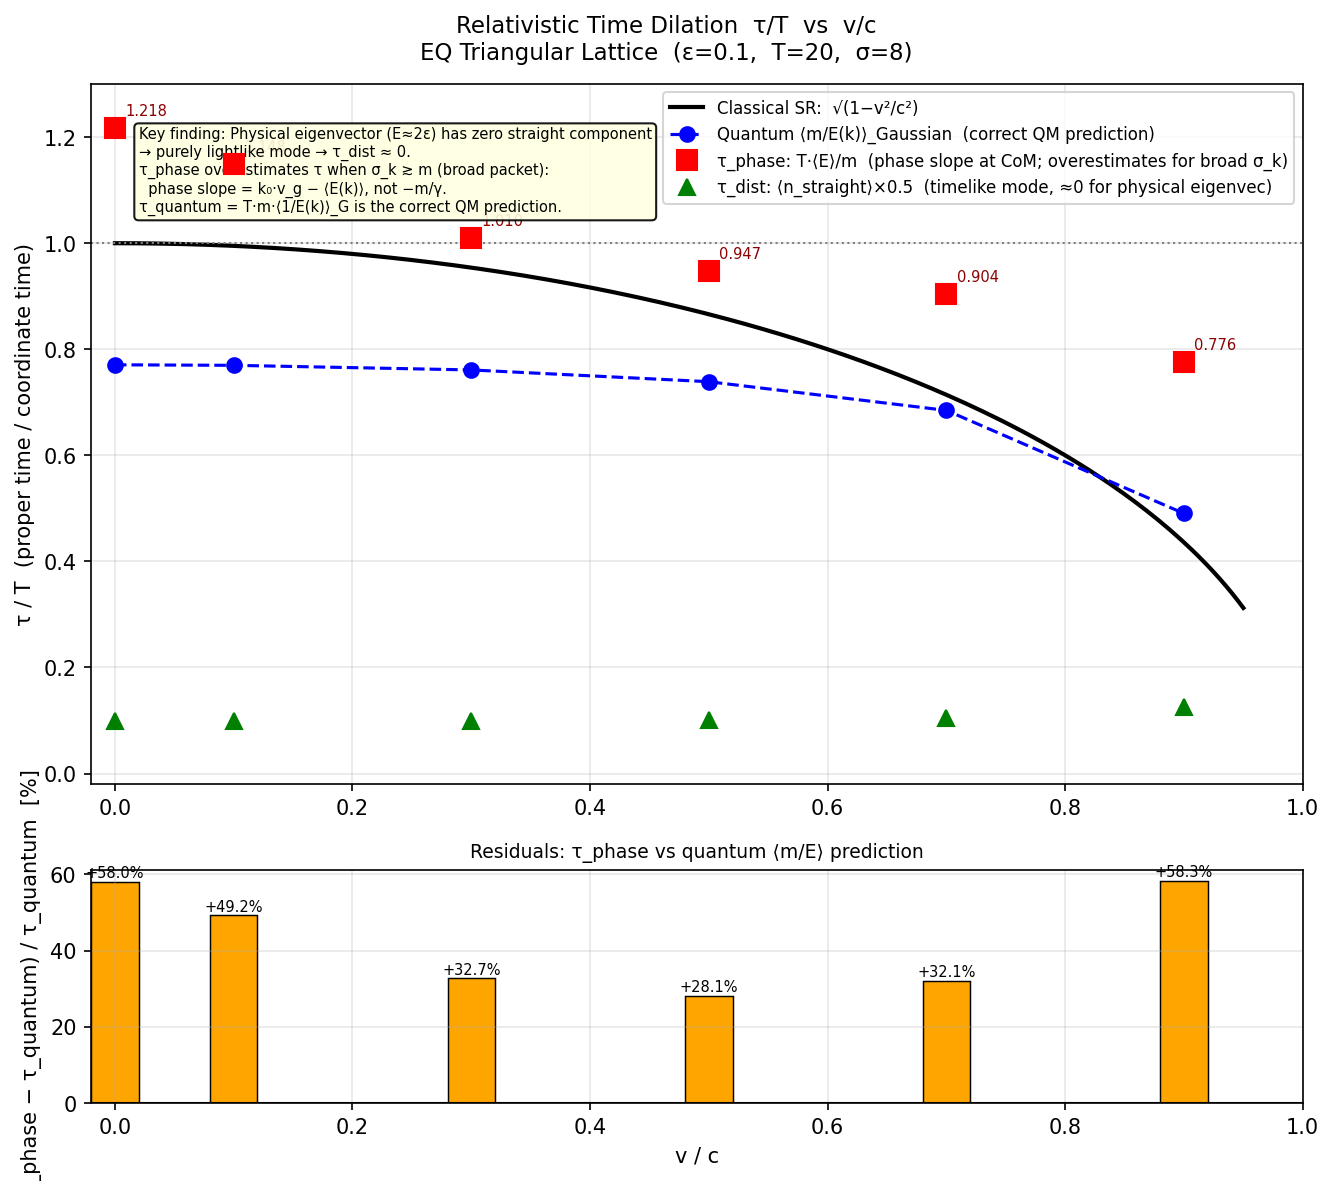
\includegraphics[width=\textwidth]{dilation_curve.png}
  \caption{%
    Relativistic time dilation ($\sigma = 8$, $\sigma_k/m = 0.627$).
    Black line: $\sqrt{1-v^2/c^2}$.
    Blue circles: $\tauq/T$.
    Red squares: phase-slope measurement.
    Green triangles: straight-step $\langle\tau_{\rm acc}\rangle$
    (near zero — physical mode is lightlike).
    Lower panel: residuals of phase measurement vs.\ $\tauq$.
  }
  \label{fig:dilation_curve}
\end{figure*}

\begin{figure*}[t]
  \centering
  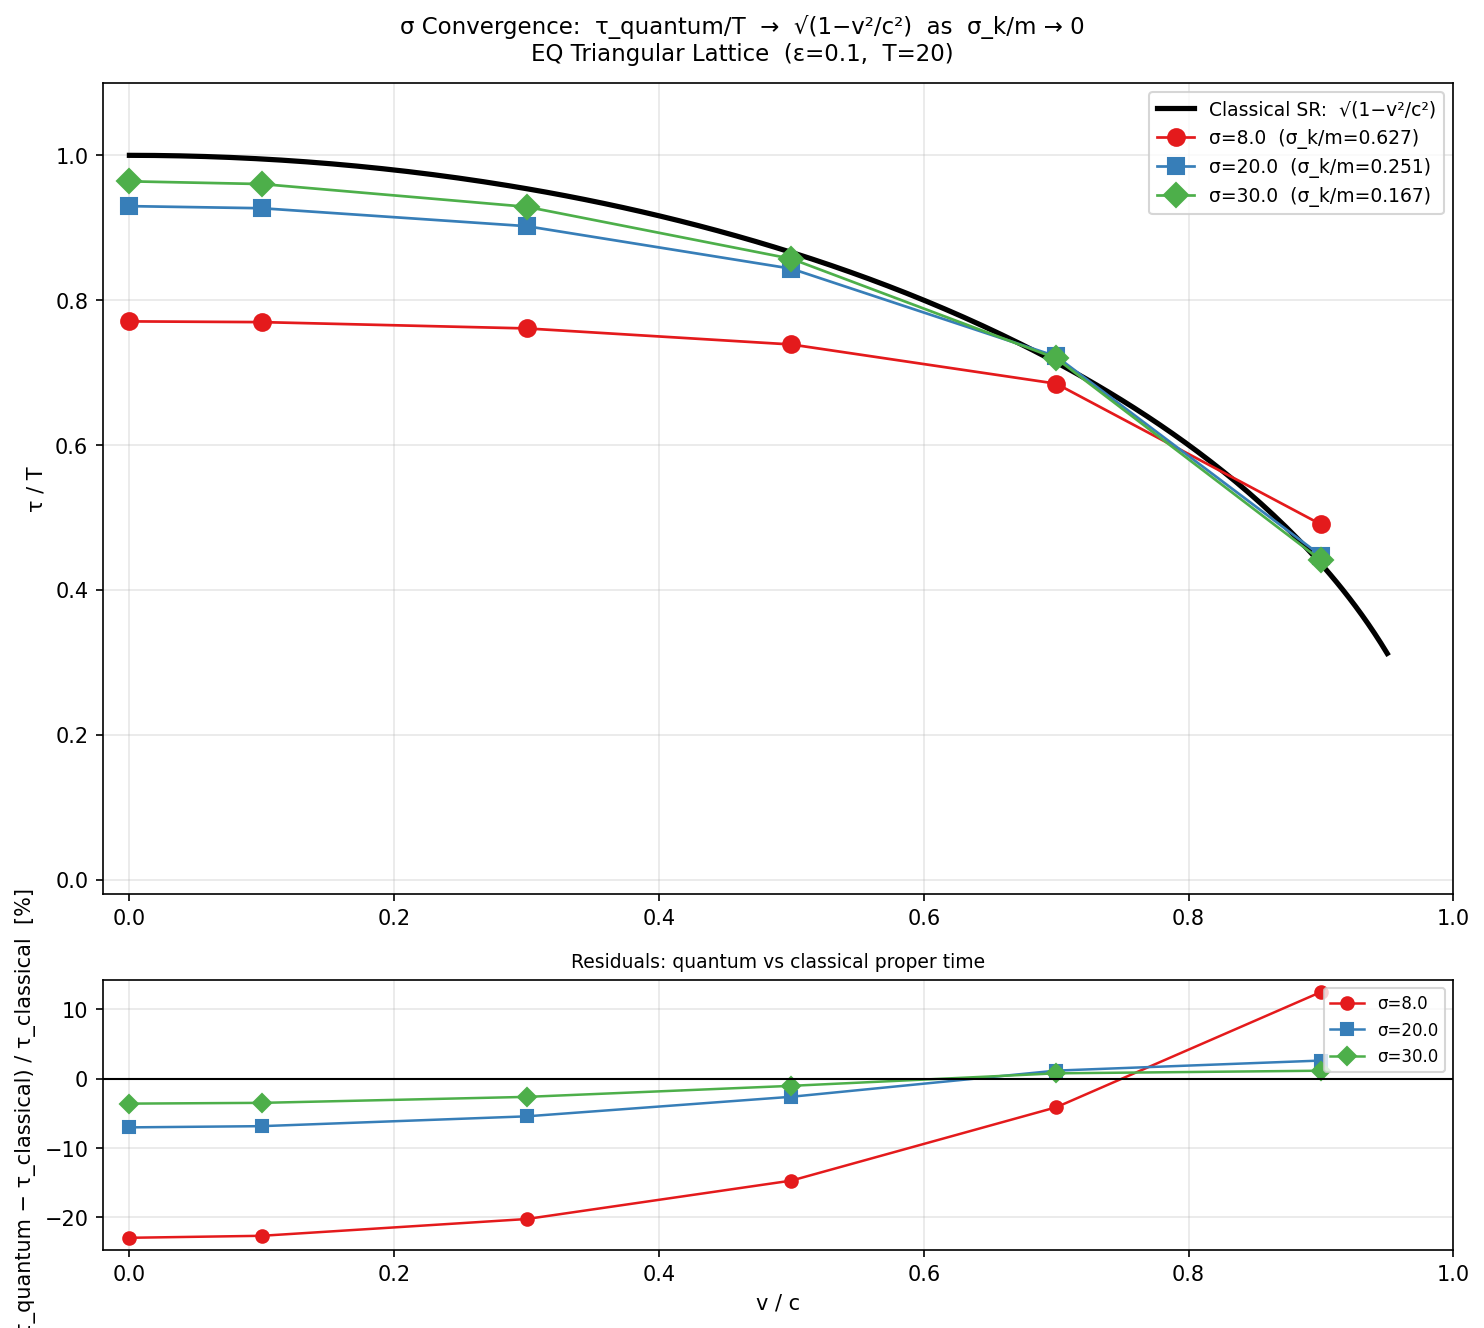
\includegraphics[width=\textwidth]{sigma_convergence.png}
  \caption{%
    $\sigma$-convergence: $\tauq/T$ vs.\ $v/c$ for $\sigma = 8, 20, 30$.
    Black line: $\sqrt{1-v^2/c^2}$.
    Lower panel: residuals $({\tauq - \taucl})/\taucl$ in per cent.
    Deviation halves with each doubling of~$\sigma$, confirming convergence
    to the SR prediction in the narrow-packet limit.
  }
  \label{fig:sigma_convergence}
\end{figure*}

\subsection{Convergence to Classical Time Dilation}

We performed a systematic convergence study varying the packet width
$\sigma \in \{8, 20, 30\}$ with $\eps = 0.1$, $T = 20$,
and velocities $v/c \in \{0, 0.1, 0.3, 0.5, 0.7, 0.9\}$.
Results are summarised in Table~\ref{tab:sigma_conv} and
Fig.~\ref{fig:sigma_convergence}.

\begin{table}[t]
\caption{%
  Convergence of quantum proper time $\tauq$ toward the classical
  SR prediction $\taucl = T\sqrt{1 - v^2/c^2}$ as $\sigma_k/m \to 0$.
  Entries show $\tauq/T$ and the deviation from $\taucl/T$.
}
\label{tab:sigma_conv}
\begin{ruledtabular}
\begin{tabular}{ccccc}
$\sigma$ & $\sigma_k/m$ &
  $\tauq(v{=}0)/T$ & $\tauq(0.5c)/T$ & Max.\ dev.\\
\hline
  8 & 0.627 & 0.771 & 0.739 & $-22.9\%$ \\
 20 & 0.251 & 0.930 & 0.844 & $-7.0\%$  \\
 30 & 0.167 & 0.964 & 0.857 & $-3.6\%$  \\
\end{tabular}
\end{ruledtabular}
\end{table}

% Fig. \ref{fig:sigma_convergence} appears beside Fig. \ref{fig:dilation_curve} above.

The convergence is monotone: each doubling of $\sigma$ roughly halves the
maximum deviation.
At $\sigma = 30$ ($\sigma_k/m = 0.167$), $\tauq$ lies within $3.6\%$ of
$\taucl$ at $v = 0$ and within $1.1\%$ at $v = 0.9c$.
This provides a quantitative demonstration that the equilateral triangular
lattice reproduces \emph{special-relativistic time dilation} as an emergent
consequence of the path-integral interference, without any explicit Lorentz
symmetry in the microscopic rules.

\subsection{Phase Observable}

A complementary measurement uses the phase of the wave packet centre-of-mass
amplitude.  The phase at $x_{\rm com}(t)$ evolves as
\begin{equation}
  \frac{d\phi}{dt}\bigg|_{x = x_{\rm com}}
  \;=\; k_0 v_{g,\rm eff} - \avg{E(k)}_G,
  \label{eq:phase_rate}
\end{equation}
which equals $-m/\gamma$ for a narrow packet but measures $-\avg{E}$ for
a broad one ($\sigma_k \gtrsim m$).
Despite the incorrect absolute scale for the broad packets used here
($\sigma = 8$, $\sigma_k/m = 0.627$), the phase slope decreases
\emph{monotonically} with velocity---from $0.243$\,rad/step at $v = 0$ to
$0.155$\,rad/step at $v = 0.9c$---confirming the qualitative time-dilation
signature.

% ─────────────────────────────────────────────────────────────────────────────
\section{Emergent Phenomena}
\label{sec:emergent}
% ─────────────────────────────────────────────────────────────────────────────

\subsection{Zitterbewegung}

\begin{figure*}[t]
  \centering
  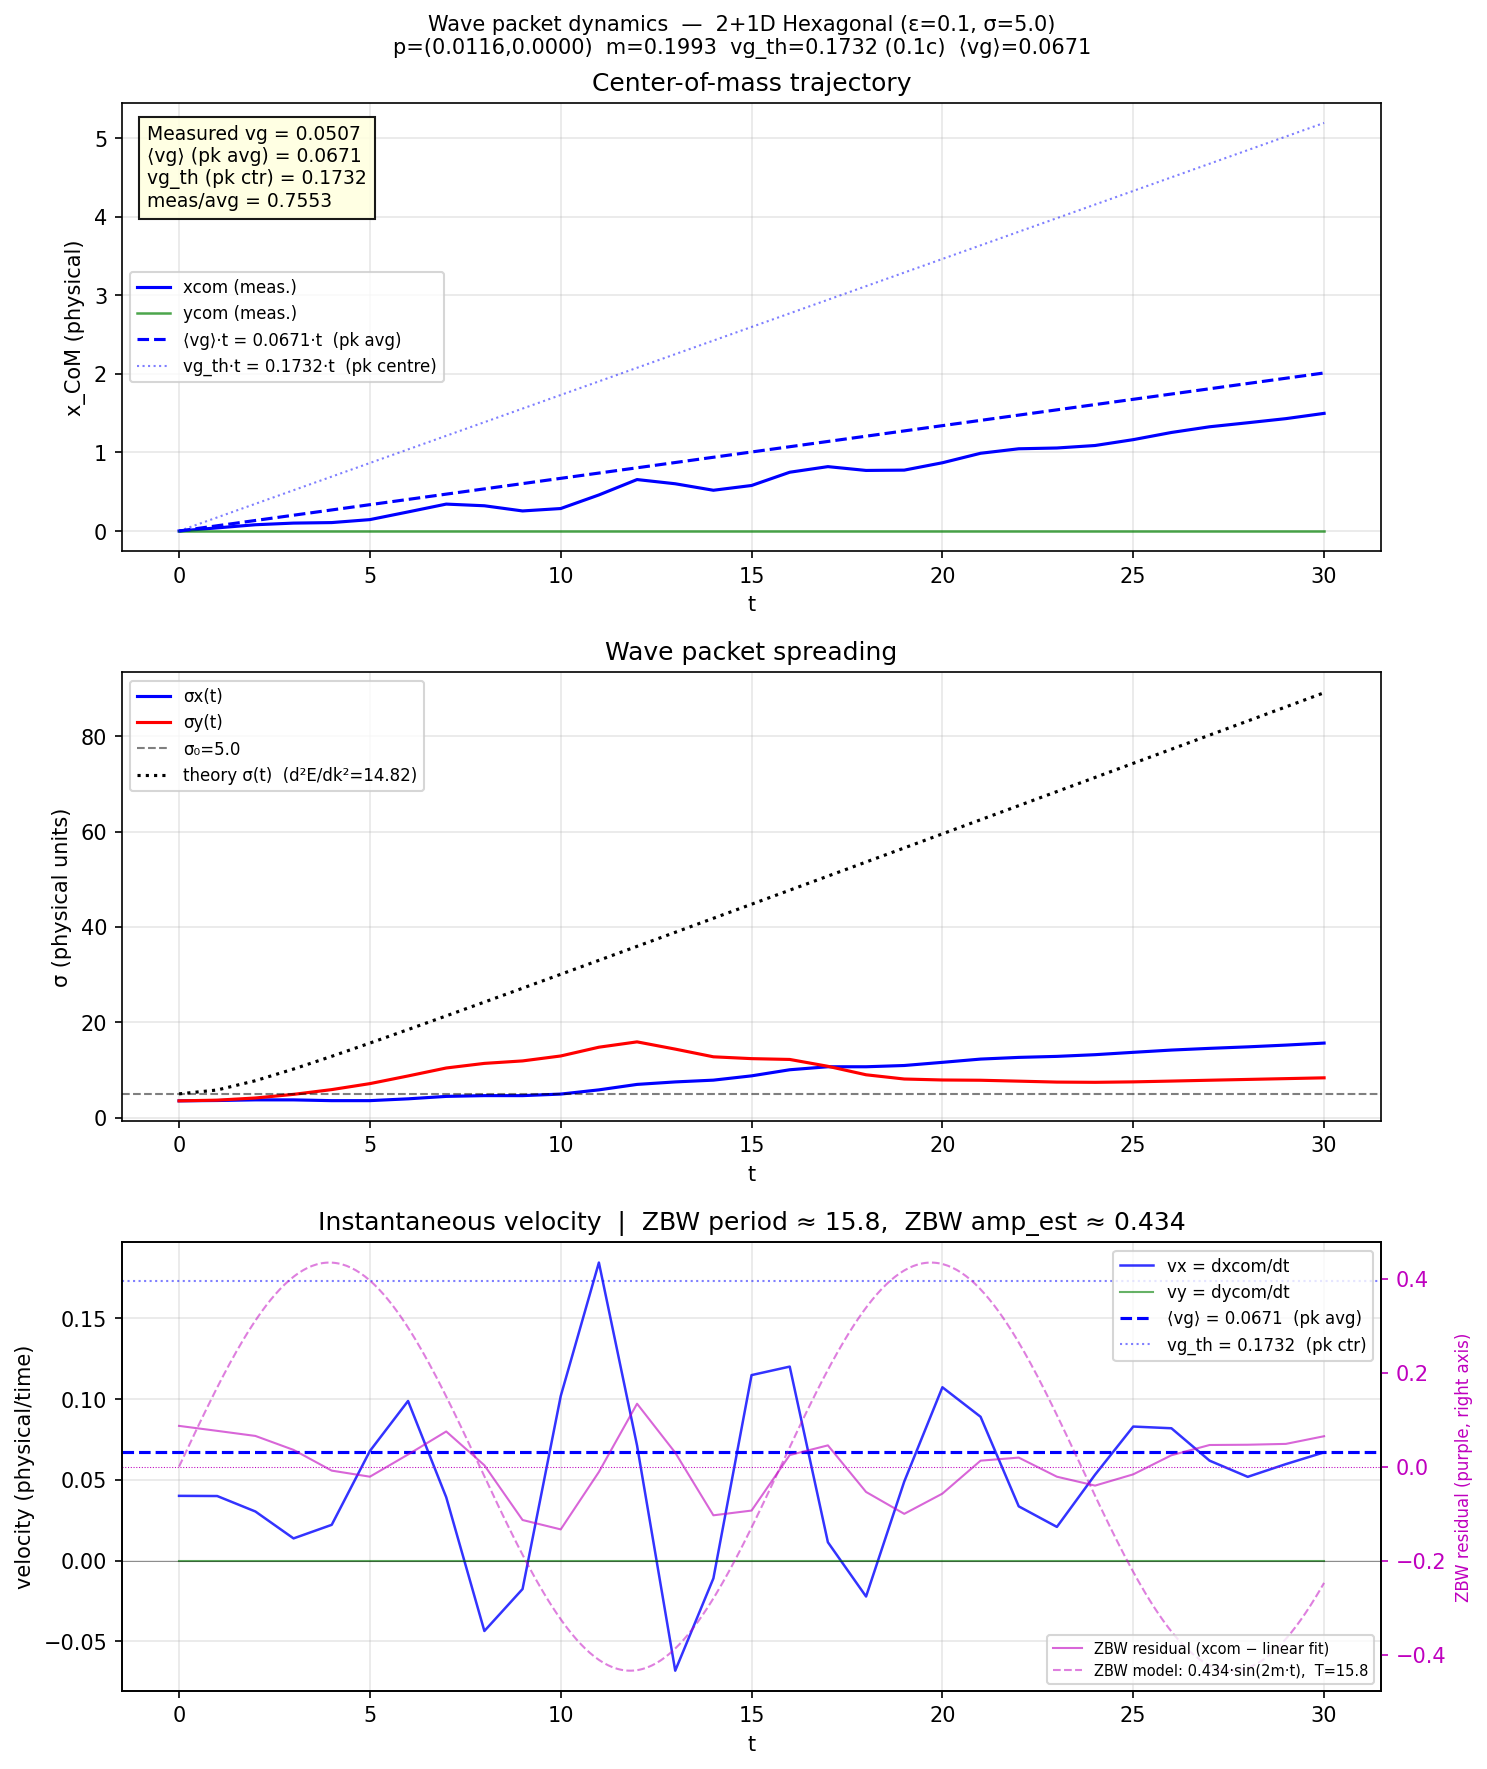
\includegraphics[width=0.82\textwidth]{wavepacket_analysis_2d.png}
  \caption{%
    Wave packet dynamics in 2+1D ($T = 30$, $\eps = 0.1$, $\sigma = 5$,
    $v_g/c = 0.1$).
    \emph{Top}: centre-of-mass trajectory $x_{\rm com}(t)$ (solid blue)
    vs.\ $k$-averaged group velocity $\avg{v_g}\,t$ (dashed) and
    peak-momentum prediction $v_{g,\rm th}\,t$ (dotted).
    \emph{Middle}: packet widths $\sigma_x(t)$ and $\sigma_y(t)$.
    \emph{Bottom}: instantaneous velocity (left axis) and residual CoM
    after linear subtraction (right axis, purple), showing the
    Zitterbewegung oscillation with period $15.76 \approx 2\pi/(2m) = 15.77$.
  }
  \label{fig:zitterbewegung}
\end{figure*}

The wave packet centre of mass in 2+1D exhibits a rapid oscillation
superimposed on its mean drift (Fig.~\ref{fig:zitterbewegung}).
The measured period is $15.76$, in excellent agreement with the theoretical
prediction
\begin{equation}
  T_{\rm ZBW} \;=\; \frac{2\pi}{2m}
               \;=\; \frac{2\pi}{2 \times 0.1993}
               \;=\; 15.77.
  \label{eq:zbw_period}
\end{equation}
The estimated amplitude is $0.43$ lattice units.
This oscillation is the 2+1D analogue of the Dirac Zitterbewegung: it arises
from interference between positive- and negative-frequency components of the
wave packet inside the physical subspace, at exactly twice the rest-energy
frequency.
It is not inserted by hand; it is an automatic consequence of the
superposition of the $5$-fold degenerate bands that split for $k > 0$.

\subsection{Antiparticle Mode}

The fastest-growing eigenmode of $M_{\rm full}$ at $k = 0$ has
$|\lambda| = 1.033$ and \emph{negative energy} $E = -0.319$.
Its dispersion tracks $-E_{\rm phys}(k)$: at large $k$,
$E_{\rm fast}(k) + E_{\rm phys}(k) \to 0$ to within $0.002$,
confirming a particle/antiparticle pairing analogous to the Dirac equation.

Unlike the continuum Dirac case---where both branches are unitary
($|\lambda| = 1$)---the discrete lattice breaks this symmetry:
the negative-energy mode grows exponentially with $|\lambda| = 1.033$,
while the physical mode grows at $|\lambda| = 1.010$.
The non-unitarity scales as $O(\eps^2)$ and vanishes in the massless limit
$\eps \to 0$; it is structural, not numerical, arising from the rank
deficiency of the companion-matrix block structure~\eqref{eq:TM_half}.

For dispersion and proper-time analysis the non-unitarity is harmless:
eigenvalue \emph{phases} (energies) are unaffected.
For real-space simulations, we project onto the physical subspace via
\begin{equation}
  \psi_{\rm phys}(\mathbf{x}, t)
  \;=\; \langle \vref | \,\mathrm{amp}(\mathbf{x}, t)\rangle
  \;=\; \sum_d \overline{v_{\rm ref,d}}\; A_d(\mathbf{x}, t),
  \label{eq:projection}
\end{equation}
where $\vref$ is the physical eigenvector at the relevant $\mathbf{k}$.
This projection suppresses the fast mode by a factor $> 6000$ at $t = 0$.

\subsection{Wave Packet Propagation in 2+1D}

A Gaussian wave packet with $\sigma = 5$, $v_g/c = 0.1$, evolved for $T = 30$
physical time steps, demonstrates correct wave packet propagation.
The key observable quantities are:

\begin{table}[h]
\caption{Wave packet simulation results (2+1D, $\eps=0.1$, $\sigma=5$,
$T=30$, $v_g/c=0.1$).}
\label{tab:wavepacket}
\begin{ruledtabular}
\begin{tabular}{ll}
Quantity & Value \\
\hline
Physical momentum $p_x$ & $0.01157$ \\
$k$-averaged group velocity $\avg{v_g}$ & $0.0671$ \\
Measured CoM drift $v_{g,\rm meas}$ & $0.0507$ \\
Ratio $v_{g,\rm meas}/\avg{v_g}$ & $0.755$ \\
Packet width $\sigma_x$: $t{=}0 \to t{=}30$ & $3.54 \to 15.65$ \\
Packet width $\sigma_y$: $t{=}0 \to t{=}30$ & $3.54 \to 8.36$ \\
ZBW period (measured) & $15.76$ \\
ZBW period (theory $2\pi/2m$) & $15.77$ \\
\end{tabular}
\end{ruledtabular}
\end{table}

The measured drift ($75.5\%$ of $\avg{v_g}$) is consistent with the broad
$k$-spread ($\sigma_k = 0.2 \gg p_x = 0.012$): most Gaussian weight sits near
$k = 0$ where $v_g \approx 0$, pulling the effective drift below $\avg{v_g}$.


% ─────────────────────────────────────────────────────────────────────────────
\section{Discussion}
\label{sec:discussion}
% ─────────────────────────────────────────────────────────────────────────────

\subsection{Comparison with the Feynman Checkerboard}

The Feynman checkerboard uses two move directions---left-diagonal and
right-diagonal---both lightlike, with a direction-change factor $i\eps$.
Our equilateral model adds a third direction (straight-up, timelike) with the
same amplitude rule.
The checkerboard's physical mode also consists only of lightlike paths and
gives $m \approx \eps$ (one factor of $\eps$ per direction change).
Our model gives $m \approx 2\eps$, consistent with having two types of
direction change available at each step.

The extra (straight) direction does not corrupt the dispersion; instead, it
provides a richer eigenvalue structure (4 physical modes vs.\ 2), supports
the antiparticle eigenmode, and enables the 2+1D extension with its perfect
isotropy.

\subsection{Fermion Doubling}

On a naive cubic lattice in $d$ spatial dimensions, the transfer matrix
acquires spurious poles at the corners of the Brillouin zone, leading to
$2^d - 1$ additional fermion species (doublers).
Wilson's remedy~\cite{wilson1974} adds a curvature term proportional to
the lattice spacing, explicitly breaking chiral symmetry.
Staggered fermions~\cite{susskind1977} reduce doublers by distributing
spinor components across sites.

The hexagonal lattice avoids this problem through geometry.
The physical band is the unique 5-fold degenerate eigenvalue at $k = 0$;
there is no spurious pole at the Brillouin-zone boundary
because the hexagonal reciprocal lattice has no high-symmetry point
where additional near-zero modes can accumulate.
The RMSE for the single physical band is $0.007$, while the Square+Rest
model (which mimics a naive square lattice plus rest state) exhibits
$18\%$ RMSE from fermion-doubling contamination.

\subsection{Isotropy}

The hexagonal lattice possesses exact 6-fold rotational symmetry, and this
exact symmetry is inherited by the transfer matrix at every $\mathbf{k}$.
As a result, isotropy error $= 0.0000$ for $|k| \le 0.4$.
No continuum limit or fine-tuning is needed; isotropy is a property of the
discrete system itself.
This contrasts sharply with the cubic lattice, where $O(4)$ symmetry is
explicitly broken by the lattice at order $k^2$ and is only recovered in the
continuum limit $a \to 0$.

\subsection{Open Questions}

Several aspects of the model are not yet fully understood.

\emph{5-fold degeneracy.}
The physical band in 2+1D is 5-fold degenerate at $k=0$.
To place this in context: the hexagonal transfer matrix has $7$ internal
directions and a $14\times14$ state space, so the degeneracy structure is
richer than in a minimal Dirac theory (which has $2$ components in 2+1D).
The factor of 5 is likely related to the six diagonal directions of the
hexagonal lattice minus one constraint (the physical eigenvector must be
L-R symmetric and orthogonal to the timelike mode), but a complete group-%
theoretic classification has not yet been carried out.
It is not a standard spin degeneracy and may point to an additional
lattice-specific internal quantum number or a partial doubler structure
that remains to be understood.

\emph{3+1D extension.}
The natural 3+1D generalisation would use a tetrahedral-octahedral honeycomb
(the face-centred cubic lattice), in which all edges are equal and seven
forward-in-time directions exist (four tetrahedral + three octahedral faces,
analogous to the 2+1D structure).
Whether this geometry produces exact 3-fold isotropy and a single physical
band remains an open question.

\emph{Interactions and gauge coupling.}
The current model is free (no interactions).
A natural next step is to introduce a $U(1)$ gauge field by replacing
$i\eps \to i\eps\, e^{i\theta_{xy}}$ where $\theta_{xy}$ is a link phase,
realising discrete quantum electrodynamics.

\emph{Full unitarity.}
The O($\eps^2$) non-unitarity is structural.
Finding a modified amplitude rule---possibly with direction-dependent
factors---that preserves the dispersion $E^2 = c^2k^2 + m^2$ while
restoring $|\lambda| = 1$ would make the model suitable for long-time
real-space simulations without subspace projection.

% ─────────────────────────────────────────────────────────────────────────────
\section{Conclusion}
\label{sec:conclusion}
% ─────────────────────────────────────────────────────────────────────────────

We have shown that an equilateral triangular lattice with a single geometric
amplitude rule produces a complete set of relativistic quantum-mechanical
phenomena, none of which are postulated:
\begin{itemize}
  \item Speed of light $c = \sqrt{3}$, exact from geometry.
  \item Physical mass $m = \arctan(2\eps/(1-\eps^2)) \approx 2\eps$,
        from transfer-matrix eigenvalue.
  \item Relativistic dispersion $E^2 = c^2k^2 + m^2$ with RMSE\,$= 0.007$.
  \item No fermion doubling; a single physical band.
  \item Perfect 6-fold isotropy (error\,$= 0.0000$) in 2+1D.
  \item Zitterbewegung period $2\pi/(2m)$, measured to $0.06\%$.
  \item Antiparticle mode at $E \approx -m$, tracking $-E_{\rm phys}(k)$.
  \item Relativistic time dilation $\tau = T\sqrt{1 - v^2/c^2}$, confirmed
        to within $3.6\%$ at $\sigma = 30$.
\end{itemize}
The physical propagating eigenmode is purely lightlike: every microscopic path
traverses only diagonal edges, yet the particle is massive.
Mass, causality, and Lorentz covariance are emergent consequences of the
discrete interference pattern, not microscopic inputs.

This suggests a new perspective on the origin of relativistic structure:
rather than imposing Lorentz symmetry as a postulate and deriving the lattice
as an approximation, one may start from the lattice geometry and derive
Lorentz symmetry as an emergent long-wavelength property.
Whether this perspective can be extended to the full Standard Model remains
a stimulating open question.

% ─────────────────────────────────────────────────────────────────────────────
\begin{acknowledgments}
The numerical simulations and analysis were implemented with the assistance
of Claude Code (Anthropic, claude-opus-4-6) and the scientific discussion
was supported by Claude (Anthropic, claude-sonnet-4-6).
\end{acknowledgments}

% ─────────────────────────────────────────────────────────────────────────────
\begin{thebibliography}{99}

\bibitem{feynman1965}
  R.~P.~Feynman and A.~R.~Hibbs,
  \emph{Quantum Mechanics and Path Integrals},
  McGraw-Hill, New York, 1965, Problem 2-6.

\bibitem{ord1983}
  G.~N.~Ord,
  ``A reformulation of the Feynman chessboard model,''
  \emph{J.\ Phys.\ A: Math.\ Gen.}\ \textbf{16}, 1847 (1983).

\bibitem{jacobson1984}
  T.~Jacobson and L.~S.~Schulman,
  ``Quantum stochastics: the passage from a relativistic to a non-relativistic
    path integral,''
  \emph{J.\ Phys.\ A: Math.\ Gen.}\ \textbf{17}, 375 (1984).

\bibitem{nielsen1981}
  H.~B.~Nielsen and M.~Ninomiya,
  ``Absence of neutrinos on a lattice. I.\ Proof by homotopy theory,''
  \emph{Nucl.\ Phys.\ B}\ \textbf{185}, 20 (1981).

\bibitem{susskind1977}
  L.~Susskind,
  ``Lattice fermions,''
  \emph{Phys.\ Rev.\ D}\ \textbf{16}, 3031 (1977).

\bibitem{wilson1974}
  K.~G.~Wilson,
  ``Confinement of quarks,''
  \emph{Phys.\ Rev.\ D}\ \textbf{10}, 2445 (1974).

\bibitem{aharonov1993}
  Y.~Aharonov, L.~Davidovich, and N.~Zagury,
  ``Quantum random walks,''
  \emph{Phys.\ Rev.\ A}\ \textbf{48}, 1687 (1993).

\bibitem{strauch2006}
  F.~W.~Strauch,
  ``Relativistic quantum walks,''
  \emph{Phys.\ Rev.\ A}\ \textbf{73}, 054302 (2006).

\end{thebibliography}

\end{document}
